\documentclass[a4paper]{article}
\usepackage{graphicx} % Required for inserting images
\usepackage{amssymb}
\usepackage{amsmath}
\usepackage{hyperref}
\usepackage{listings}
\usepackage{fancyhdr}
\usepackage{xcolor}
\usepackage{geometry}
\usepackage{ragged2e}
\usepackage{subcaption}
\usepackage{multirow}
\usepackage{tabularx}
\usepackage{indentfirst}
\usepackage{lscape}
\usepackage{titlesec}
\usepackage[nottoc,numbib]{tocbibind}
\usepackage[usenames, dvipsnames]{xcolor}
\usepackage{tikz} \usetikzlibrary{calc}


\geometry{margin=1in}

\colorlet{myGreen}{green!70!black}
\colorlet{myDGreen}{green!50!black}
\colorlet{myGray}{white!60!black}

\newcommand{\colNaN}[1]{{\textcolor{black!30}{#1}}}
\newcommand{\colDisaster}[1]{{\textcolor{red!60}{#1}}}
\newcommand{\colFailure}[1]{{\textcolor{orange}{#1}}}
\newcommand{\colWorse}[1]{\textcolor{orange!60}{#1}}
\newcommand{\colSimilar}[1]{\textcolor{black!60}{#1}}
\newcommand{\colBetter}[1]{\textcolor{blue!70}{#1}}
\newcommand{\colSuccess}[1]{\textcolor{black!30!green}{#1}}
\newcommand{\colAmazing}[1]{\textcolor{green}{#1}}

\hypersetup{
    colorlinks,
    linkcolor={blue!50!black},
    citecolor={blue!50!black},
    urlcolor={blue!80!black}
}

\lstdefinestyle{mystyle}{
    language=Python,
    backgroundcolor=\color{white!95!black},   
    %commentstyle=\color{},
    %keywordstyle=\color{},
    %numberstyle=\tiny\color{codegray},
    %stringstyle=\color{codepurple},
    basicstyle=\ttfamily\footnotesize,
    breakatwhitespace=false,         
    breaklines=true,                 
    %captionpos=b,                    
    keepspaces=true,                 
    %numbers=left,                    
    %numbersep=5pt,                  
    showspaces=false,                
    showstringspaces=false,
    showtabs=false,                  
    tabsize=4,
}
\lstset{
    style=mystyle,
    %emph={sage},
    %emphstyle={\color{myGreen}}
}



%\renewcommand\footnoterule{\rule{.4\textwidth}{0.2pt}}
\renewcommand\footnoterule{\kern-3pt \hrule  \kern 2.6pt}
\fancyhead[L, C]{}
\fancyfoot[C]{\thepage}
\pagestyle{fancy}

\title{Internship report}
\author{Marie BONBOIRE}
\date{}

\begin{document}

\thispagestyle{plain}
\begin{titlepage}
    \begin{figure}[h]
        \centering
        
\includegraphics[width=0.4\textwidth]{su.png}
    \end{figure}
    \vspace{1cm}

    \begin{center}
        {\LARGE PCCA}\\[0.3cm]
        \rule{\linewidth}{0.5mm} \\[0.4cm]
        {\huge \textbf{Modular arithmetic and vectorization using\\ SIMD and AVX}}\\[0.4cm]
        \rule{\linewidth}{0.5mm} \\[1cm]
        {\large 24 January 2025 - ?? May 2025}\\[3cm]

        {\Large Damien ASSIRE \& Marie BONBOIRE}


    \end{center}

    \vfill
\begin{flushleft}{\large
    \textbf{Supervisor:} Mr. Vincent NEIGER\footnote{\url{https://vincent.neiger.science/}} (LIP6 - PolSys)\\
    }
\end{flushleft}
\end{titlepage}
\newpage

\tableofcontents
\newpage

\section{Preface}

\subsection{Goals}
\begin{itemize}
    \item Implement basic arithemic operations (scalar-vector multiplication, vector-vector multiplication, dot product) using Flint.
    \item Study the impact of the modulo operation.
    \item Enhance these operations using Intel's intrinsics for Single Instruction Multiple Datas (SIMD) vectorization.
    \item Advanced benchmarking/profiling.
    \item Apply on a form of butterfly FFT for a forward integration to Flint.
\end{itemize}

\subsection{Machines description}


% 2023 - 4.5 GHz % mariz
% 2019 - 2.5 GHz % ppti
% 2023 - 3.3 GHz % argiope
% 2021 - 3.0 GHz % groebner

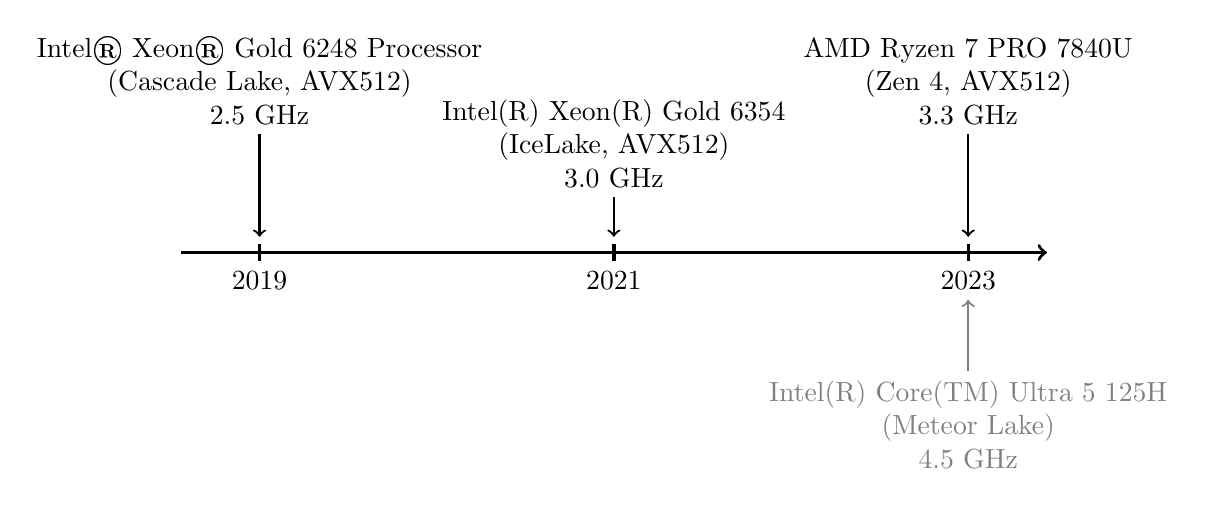
\begin{tikzpicture}[very thick, black]

    %coordinates
    \coordinate (O) at (1,0); % Origin
    \coordinate (F) at (12,0); %End
    \coordinate (P1) at (2,0); %ppti
    \coordinate (P2) at (6.5,0); %groebner
    \coordinate (P3) at (11,0); %mariz+argiope

    %proc
    \draw[<-,thick,color=black] ($(P1)+(0,0.2)$) -- ($(P1)+(0,1.5)$) node [above=0pt,align=center,black] 
    {Intel® Xeon® Gold 6248 Processor \\ (Cascade Lake, AVX512) \\ 2.5 GHz};
    \draw[<-,thick,color=black] ($(P2)+(0,0.2)$) -- ($(P2)+(0,0.7)$) node [above=0pt,align=center,black] 
    {Intel(R) Xeon(R) Gold 6354 \\ (IceLake, AVX512) \\ 3.0 GHz};
    \draw[<-,thick,color=black] ($(P3)+(0,0.2)$) -- ($(P3)+(0,1.5)$) node [above=0pt,align=center,black] 
    {AMD Ryzen 7 PRO 7840U \\ (Zen 4, AVX512) \\ 3.3 GHz};
    \draw[<-,thick,color=gray] ($(P3)-(0,0.6)$) -- ($(P3)-(0,1.5)$) node [below=0pt,align=center,gray] 
    {Intel(R) Core(TM) Ultra 5 125H \\ (Meteor Lake) \\ 4.5 GHz};

    %main arrow
    \draw[->] (O) -- (F);

    %ticks
    \foreach \x in {2,6.5,11}
    \draw(\x cm,3pt) -- (\x cm,-3pt);
    %labels
    \foreach \i \j in {2/2019,6.5/2021,11/2023}{
    	\draw (\i,0) node[below=3pt] {\j} ;
    }

\end{tikzpicture}

\section{SIMD instructions}

\begin{itemize}
    \item Intel intrinsics guide\footnote{\url{https://www.intel.com/content/www/us/en/docs/intrinsics-guide/index.html}}
    \item avx2: 256 bits registers \texttt{\_\_m256i} --> vectors of 4 integers
    \item avx512: 512 bits registers \texttt{\_\_m512i} --> vectors of 8 integers
    \item general description cf. slides PPAR
\end{itemize}


\section{Multiplication of 64 bits integers}

When multiplying two integers, a problem of overflow can arise since the result might be too big to be stored in a 64 bits word. 
To circumvent this issue, one needs to first split the two integers into two words of a given size and then apply the long multiplication.

\subsection{Long multiplication}
Given two integers $a$ and $b$ both of at most 64 bits, we start by splitting them into 2 words, one of $k$ bits and the other one of at most $64-k$ bits, with $k<64$:

\begin{align*}
    a &= a_{hi}\cdot 2^{k} + a_{lo} \\
    b &= b_{hi}\cdot 2^{k} + b_{lo}.
\end{align*}

The long multiplication consists in computing the multiplication of 64 bits limbs using multiplications and additions of integers with a lower size.

We compute
\begin{align*}
    r_{lo} &= a_{lo}\cdot b_{lo} \\
    r_{mi} &= a_{lo}\cdot b_{hi} + a_{hi}\cdot b_{lo} \\
    r_{hi} &= a_{hi}\cdot b_{hi}
\end{align*}
then $ab = r_{lo} + (r_{mi} \ll k) + (r_{hi} \ll 2k)$.


\subsection{Retrieve the high and the low part of the result}

Since the product $ab$ can have more than 64 bits, the output of this operation is usually given as a pair of words of at most 64 bits such that $ab = (ab)_{hi}\cdot 2^{64} + (ab)_{lo}$.

\begin{itemize}
    \item Flint's function \texttt{umulppmm}
    \item avx2: no mullo/mulhi
    \item avx512: mullo but no mulhi
\end{itemize} 

\section{Classic arithemic operations on vectors}

\subsection{Addition of two vectors}

\begin{itemize}
    \item not done atm but todo 
    \item modular reduction might be delayed
\end{itemize}

\subsection{Multiplication of a vector by a scalar or by another vector}

\begin{itemize}
    \item define the operations.
    \item boils down to mult described above
\end{itemize}

\subsection{Dot product}

For two vectors $u$ and $v$ of $len$ integers of bit size $bitsize \le 32$, and an integer $n$ of some bit size, we want to compute

\[\left(\sum_{i=0}^{len}u_iv_i\right) \mod n\]

To compute the sum of products, we split the integers as described in subsection \ref{sub:split}. Then, we sum separately the three limbs $r_{high}$, $r_{mid}$, $r_{low}$. % TODO: Verify name

\subsubsection{Modular reduction}

The modular is done with \texttt{NMOD2\_RED2} from the flint library. We first regroup the three limbs in two limbs $h$ and $l$ as follows:

\begin{align}
    l &= r_{mid}B &+ \left(r_{high}B^2 + r_{low}\right) \\
    h &= \left\lfloor r_{mid}\frac{B}{2^{64}}\right\rfloor &+ \left\lfloor r_{hi}\frac{B^2}{2^{64}}\right\rfloor &+ c \quad{\text{where $c$ is $1$ if the computation of l overflows and 0 otherwise}}
\end{align}

Because of the cost of this operation, we only reduce at the end, adter the sum. As a consequence, the number of integers we can sum without overflows is limited, and depend of their size.

\begin{proposition}\label{prop:sum}
    For integers of size $\S$, the result of the sum of $2^n$ of such integers is at most $S + n$
\end{proposition}

\begin{proof}
    By induction on $n\in\mathbf{N}$

    \paragraph{Base case: $n = 0$}
    $2^0 = 1$, thus no addition is done and the result has size $S = S + 0 = S + n$. Hence, $\Pi(0)$ is verified.

    \paragraph{Induction}
    Assume for some $i \in \mathbf{N}^*$, $\Pi(i - 1)$ is verified.

    Let $u$ and $v$ be the sums of $2^{i-1}$ integers of size $ S $. By $\Pi(i-1)$, their sizes are at most $S + i - 1$. So the size of $u + v$ is at most $\left(S + i + 1\right) + 1 = S + i$, and $u + v$ is the sum of $2 \cdot 2^(i-1) = 2^i$ integers.
    So $\Pi(i)$ is verified, hence $\Pi(i-1) \Rightarrow \Pi(i)$

    \paragraph{By induction's principle:} $\Pi(0)$ is verified and $\forall i\in\mathbf{N},\ \Pi(i) \Rightarrow \Pi(i+1)$, So
    \begin{displaymath}
        \forall n\in\mathbf{N},\ \Pi(n)\text{ is verified}
    \end{displaymath}
\end{proof}

This value can be computed using \ref{prop:sum}. In our case, because we sum the results of the products of two integers of bit size $bitsize,\ S = 2 bitsize$.

TODO: Max for rhi, rmi and rlo



\section{Butterfly fft}
\begin{align*}
    add &= a + w*b \mod n \\
    sub &= a - w*b \mod n 
\end{align*}

\subsection{Shoup's multiplication}


\paragraph{Motivations:} Compute repeated multiplications with fixed $a$ and $n$, and varying $b$ => w*b

steps:
\begin{enumerate}
    \item find $p_{hi}, p_{lo}$ such that $w_{pre} * b = p_{hi}W + p_{lo}$,
    \item compute $c = wb - p_{hi}n$
    \item if $c \leq n$, return $c-n$ else return $c$.
\end{enumerate}

The correctness of this algorithm relies on the definition of $w_{pre}$. 

\begin{proposition}\label{prop:quorem}
For $(a,b) \in \mathbb{Z}\times \mathbb{N}^*$, the quantities $q=\left\lfloor\frac{a}{b}\right\rfloor$ and $r=a - \left\lfloor\frac{a}{b}\right\rfloor b$ are respectively the quotient and the remainder in the Euclidian division of $a$ by $b$.
\end{proposition}
    
\begin{proof}
From the definition of the floor of a rational number, we have:
\[
    \left\lfloor\dfrac{a}{b}\right\rfloor \leq \dfrac{a}{b} < \left\lfloor\dfrac{a}{b}\right\rfloor \Longleftrightarrow
    \left\lfloor\dfrac{a}{b}\right\rfloor b \leq a < \left\lfloor\dfrac{a}{b}\right\rfloor b + b \Longleftrightarrow
    0 \leq a - \left\lfloor\dfrac{a}{b}\right\rfloor b < b.
\]
We then consider $q=\left\lfloor\dfrac{a}{b}\right\rfloor$ and by the uniqueness of the quotient in the Euclidian division with remainder, it implies that $a = bq + r$ with $r=a - \left\lfloor\dfrac{a}{b}\right\rfloor b$ and $0 \leq r < b$.
\end{proof}

\begin{proof} (Correctness of the algorithm)
First, using \autoref{prop:quorem}, we have that $w_{pre}= \left\lfloor\frac{wB}{n}\right\rfloor $ is the quotient in the division of $wB$ by $n$. Thus,
\begin{align*}
wB &= w_{pre}\cdot n + r \text{ with } 0 \leq r < n \\
w_{pre} &= \dfrac{wB - r}{n}
\end{align*}
Thus, by definition of $p_{hi}$,
\[
p_{hi} = \left\lfloor\frac{w_{pre}\cdot b}{B}\right\rfloor
= \left\lfloor\dfrac{wb}{n} - \dfrac{rb}{nB} \right\rfloor.
\]

From the requirements on $r$ ($<n$) and $b$ ($<B$), and the previous result, we have that
\[
\left\lfloor\dfrac{wb}{n}\right\rfloor - 1 \leq p_{hi} \leq \left\lfloor\dfrac{wb}{n}\right\rfloor
\]
and this means that $p_{hi}$ is either $\left\lfloor\frac{wb}{n}\right\rfloor - 1$ or $\left\lfloor\frac{wb}{n}\right\rfloor$.


It follows that 
\begin{align*}
\text{either } &c=w\cdot b - \left\lfloor\frac{wb}{n}\right\rfloor n + n \\
\text{or } &c=w\cdot b - \left\lfloor\frac{wb}{n}\right\rfloor n.
\end{align*}
Using \autoref{prop:quorem} again, we have $c=wb \mod n$ or $c=(wb \mod n)+n$, and the last step of the algorithm ensures that we retrieve $wb \mod n$.
\end{proof}

\subsection{Harvey's lazy butterfly fft}

\begin{itemize}
    \item restrict the size of the inputs such that the output can be stored in a 64 bits word.
    \item describe theses restrictions.
\end{itemize}


\section{Modular reduction with special primes}

\subsection{Mersenne primes}

$p = 2^x - 1$
\[
p \mod p \Longleftrightarrow 2^x - 1 = 0 \mod p \Longleftrightarrow 1^u = 1 \mod p
\]
------> with $ab = ab_{hi}\cdot 2^{64} + ab_{lo}$, it means that if we take the Mersenne's prime number $p = 2^{64} - 1$, we can compute $ab \mod p$ with only one addition 
\[
    ab \mod p \Longleftrightarrow ab_{hi}\ + ab_{lo} \mod p
\]



\section{Profiling/Benchmarking}



\subsection{Verification of timings}

\subsection{Impact of caches} % todo Draft

In the benchmarks, we observes bigger factors than expected between two sizes,
e.g. during the unrolling of non modular dot product. This happen when a vector
become too big to fit in a certain cache, and must be stored in a lower level
cache or in the primary memory. In the previously cited case, it happen for sizes
65536 and 131072 on ppti-gpu-4. % todo detail of calculation


\subsection{Results}

\section{Conclusion}



\newpage
\bibliographystyle{plain} 
\bibliography{biblio} 
\nocite{*}

\end{document}
